% !TEX spellcheck = en-US
\chapter{Sensor Fusion Involving Inertial Sensors}
\label{cha:applications} 
In this tutorial, we have presented a number of algorithms and modeling possibilities for position and orientation estimation using inertial sensors. The algorithms derived in \Chapterref{cha:orientationEstimation} are based on the simple state space models~\eqref{eq:models-ssPose} and~\eqref{eq:models-ssOri}. These models assume the availability of inertial measurements supplemented with either magnetometer or position measurements. In this chapter, we will illustrate how the same or similar algorithms can be used when additional and/or different supplementary sensors are available and discuss a number of possible extensions. The models used in this chapter will be more complex, but the information provided by the inertial sensors will remain one of the basic building blocks. We are not aiming for a full coverage, since that would require too much space. Instead we provide a number of case studies to illustrate what can be done when it comes to including the developments from Chapters~\ref{cha:introduction}--\ref{cha:calibration} into a more complex setting. The case studies are the modeling of a non-Gaussian noise distribution to make use of radio-based time of arrival measurements (\Sectionref{sec:appl-uwb}), the fusion of information from inertial sensors with cameras (\Sectionref{sec:appl-vision}), and motion capture based on information from multiple inertial sensors in combination with information about the human motion (\Sectionref{sec:appl-motionCapture} and \Sectionref{sec:appl-actRecogn}).

\section{Non-Gaussian noise distributions: time of arrival measurements}
\label{sec:appl-uwb}
In the algorithms presented in \Chapterref{cha:orientationEstimation}, we assumed that the measurement noise of the sensors is properly described using a Gaussian distribution. This was shown to be a fair assumption for the inertial measurement noise based on experimental data in \Exampleref{ex:sensors-inertialMeasurements}. In this section we will illustrate the possibility of modeling non-Gaussian measurement noise using a practical example. We will also describe possible adaptations of the algorithms presented in \Chapterref{cha:orientationEstimation} to incorporate non-Gaussian noise models. 

\begin{figure}
	\centering
		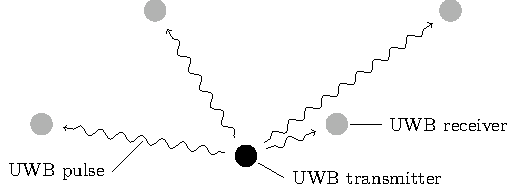
\includegraphics[scale = 1]{figure6_1.pdf}
  \caption{A \gls{uwb} setup consisting of a number of
    		stationary receivers obtaining \acrlong{toa} measurements of
    		signal pulses originating from a mobile transmitter.}
  \label{fig:appl-uwb-uwbSetup}
\end{figure}

In the state space model~\eqref{eq:models-ssPose}, we assumed the presence of position measurements with additive Gaussian noise. Many sensors, however, do not directly measure the position, see \eg \cite{gustafssonG:2005}. An example of a type of measurements that can be obtained are \emph{\gls{toa}} measurements from a \gls{uwb} system. These \gls{toa} measurements provide information about when a radio pulse sent out by a mobile transmitter arrives at a stationary receiver. This is graphically illustrated in \Figureref{fig:appl-uwb-uwbSetup}. These types of measurements can be modeled as
\begin{align}
  \label{eq:appl-uwb-measModel}
  y_{\text{u},mk} = \tau_{k}
    + \tfrac{1}{c} \| r_m - t_{k} \|_2 
    + \Delta\tau_m
    +   e_{\text{u},mk}.
\end{align}
Here, $c$ denotes the speed of light, $t_{k}$
is the position of the transmitter at the time of transmitting the $k^\text{th}$ pulse,
$r_m$ is the position of the $m^\text{th}$ receiver and $\Delta\tau_m$ is its clock-offset. The time when pulse $k$ is transmitted is denoted by $\tau_{k}$. Finally, $e_{\text{u},mk}$ is measurement noise. 

Using time of arrival measurements from a number of receivers it is possible to compute the position of the transmitter at the time when the pulse was sent. In many applications, the mobile transmitters have a much less accurate clock than the stationary receivers and $\tau_{k}$ is therefore assumed to be an unknown variable to be estimated. For a setup with $M$ stationary transmitters, the position of the transmitter when transmitting the pulse $k$ and the time when the pulse was transmitted can be estimated using multilateration~\citep{chanH:1994, geziciTGKMPS:2005,sayedTK:2005, sahinogluGG:2008}. 

Due to \acrlong{nlos} conditions and/or multipath we expect a small number of measurements to be delayed. In~\cite{kokHS:2015}, we present an approach that models the measurement noise $e_{\text{u},mk}$ using a tailored asymmetric heavy-tailed distribution. Here, a heavy-tailed Cauchy distribution allows for measurement \textit{delays}, while a Gaussian distribution excludes the physically unreasonable possibility of pulses traveling faster than the speed of light as
\begin{subnumcases}{\label{eq:appl-uwb-noiseMeasModel} e_{\text{u},mk} \sim}
\left( 2 - \alpha \right) \mathcal{N}(0,\sigma^2)  & for $e_{\text{u},mk} < 0$, \\
\alpha \, \text{Cauchy}(0,\gamma) & for $e_{\text{u},mk} \geq 0$. 
\end{subnumcases}
The presence of the constants $\alpha$ and $2 - \alpha$ is motivated by the fact that the proposed asymmetric probability density function needs to integrate to one. The parameter $\alpha$ is defined as a function of $\sigma$ and $\gamma$. The proposed asymmetric probability density function and its corresponding negative log-likelihood, given by
\begin{subnumcases}{\label{eq:appl-uwb-negLogLik} - \log p \left( e_{\text{u},mk} \right)=}
\mathcal{L}_G & for $e_{\text{u},mk} < 0$,\\
\mathcal{L}_C & for $e_{\text{u},mk} \geq 0$, 
\end{subnumcases}%
\begin{align*}
\mathcal{L}_G &\triangleq \tfrac{e_{\text{u},mk}^2}{2 \sigma^2} + \tfrac{1}{2} \log \sigma^2 + \tfrac{1}{2} \log 2 \pi - \log \left( 2 - \alpha \right), \\
\mathcal{L}_C &\triangleq \log \left( 1 + \tfrac{e_{\text{u},mk}^2}{\gamma^2} \right) + \tfrac{1}{2} \log \gamma^2 + \log \pi - \log \alpha,
\end{align*}
are both depicted in \Figureref{fig:appl-uwb-loglikelihood} in red. For comparison, the Gaussian and Cauchy probability density functions are also depicted, in blue and green, respectively. Related studies have also modeled this presence of delayed measurements using skew-$t$ distributions \citep{nurminenAPG:2015,mullerPRS:2016}, Gaussian mixture models \citep{mullerWP:2014} or by introducing a number of unknown delays~\cite{hol:2011}.

\begin{figure}
	\centering
	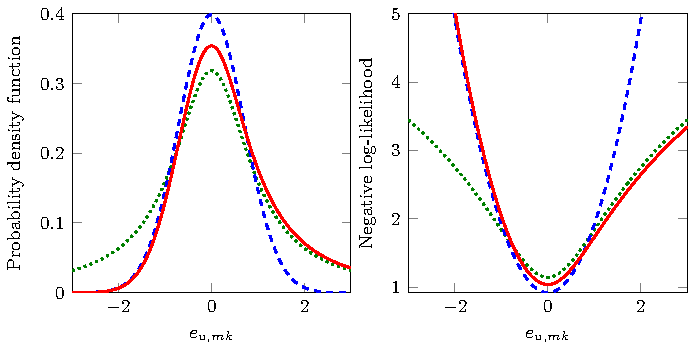
\includegraphics[scale = 1]{figure6_2.pdf}
		\caption{Probability density function (left) and negative log-likelihood (right) of a $\mathcal{N}(0,1)$ distribution (blue, dashed), a $\text{Cauchy}(0,1)$ distribution (green, dotted) and the asymmetric distribution~\eqref{eq:appl-uwb-noiseMeasModel} assuming $\sigma = \gamma = 1$ (red).}
	\label{fig:appl-uwb-loglikelihood}
\end{figure}

The filtering and smoothing algorithms posed as optimization problems, see \Sectionref{sec:oriEst-smoothingOpt} and \Sectionref{sec:oriEst-filteringOpt}, can straightforwardly be adapted to include the asymmetric probability density function by using~\eqref{eq:appl-uwb-negLogLik} in the objective function instead of the weighted least squares term representing the measurement model, see \eg \eqref{eq:oriEst-posSmoothing}. Extended Kalman filters intrinsically assume that the process and measurement noise are Gaussian. For the extended Kalman filters implementations presented in \Sectionref{sec:oriEst-quat-ekf} and \Sectionref{sec:oriEst-oriError-ekf}, the extension to non-Gaussian noise is therefore less straightforward. Adaptations of the Kalman filter to non-Gaussian noise are, however, possible, see \eg \cite{rothAOG:2017} and the references therein for a discussion on Kalman filtering in the presence of student's $t$ distributed noise.

\section{Using more complex sensor information: inertial and vision}
\label{sec:appl-vision}
In the model~\eqref{eq:models-ssPose}, we assumed that a sensor directly measuring the position was available. In \Sectionref{sec:appl-uwb}, we instead considered the case of \gls{toa} measurements from a \gls{uwb} system. In this section, we will focus on pose estimation using a camera and an \gls{imu} that are rigidly attached to each other. Inertial sensors and camera images have successfully been combined for pose estimation, see \eg \cite{brysonJS:2009,luptonS:2012,jungT:2001,sjanicSG:2017,leuteneggerLBSF:2015,forsterCDS:2016,bleserS:2009,foxlinN:2003,nyqvistG:2013}. Application areas are for instance robotics, \acrlong{vr} and \acrlong{ar}.

To use camera images of the environment of the sensor to provide information about where the sensor is located in this environment, a number of \emph{features} is typically extracted from each image. These features are subsequently associated with a point in the environment. Advanced feature extraction and association algorithms are available, see \eg \cite{harrisS:1988,bayTG:2006,lowe:2004,fischlerB:1981}. 

\begin{figure}
  	\centering
    	\subfigure[Illustration of the pinhole camera model where an object $l$ results in an image $i$ in the image plane. The image plane lies a distance $f$ behind the pinhole.]{
	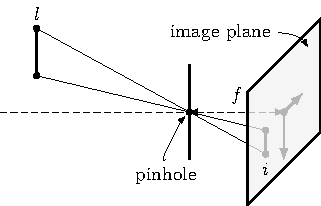
\includegraphics[scale = 1]{figure6_3a.pdf}
	\label{fig:appl-vision-pinhole}}
    	\subfigure[2D visualization of the relation between the position of the point $l$ with respect to the pinhole and the position of its image $i$.]{
	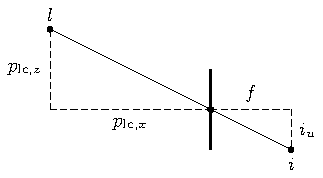
\includegraphics[scale = 1]{figure6_3b.pdf}
	\label{fig:appl-vision-pointProj}}	
    	\caption[]{Illustrations of the relation between a point or object $l$ in the environment and its image $i$.}
    	\label{fig:appl-vision}
\end{figure}

To be able to use the features and their associated points in the real world for pose estimation, a model is required that relates points in the image to the environment. A simple model that can be used for this is a pin-hole model. Such a model is illustrated in \Figureref{fig:appl-vision-pinhole}, where an object $l$ results in an image $i$ in the image plane. The size of $i$ depends on the size of the object, the distance of the object to the pinhole and on the \emph{focal length}~$f$. The focal length is an intrinsic property of a camera and is typically assumed to be known. 

Let us now assume that the object $l$ is simply a point and denote its position with respect to the pinhole center by $p_{\text{lc}} = \begin{pmatrix} p_{\text{lc},x} & p_{\text{lc},y} & p_{\text{lc},z} \end{pmatrix}^\Transp$. We denote the position of the object $l$ in the image frame by $i = \begin{pmatrix} i_u & i_v \end{pmatrix}$. A two-dimensional illustration of this can be found in \Figureref{fig:appl-vision-pointProj}. The position $i$ can be expressed in terms of $p_{\text{lc}}$ and the focal length $f$ as
\begin{align}
\label{eq:appl-imPoints}
\begin{pmatrix} i_{u} \\ i_{v} \end{pmatrix} = f
\begin{pmatrix} \tfrac{p_{\text{lc},z}^\text{c}}{p_{\text{lc},x}^\text{c}} & \tfrac{p_{\text{lc},z}^\text{c}}{p_{\text{lc},y}^\text{c}} \end{pmatrix}^\Transp.
\end{align}
Here, the superscript $c$ indicates that the position $p_{\text{lc}}$ is expressed in the \emph{camera frame} $c$. The origin of the camera frame is located at the pinhole and its axes are aligned with the image plane. It is possible to express the position $p_{\text{lc}}$ in terms of the position of the camera and the position of the object $l$ as
\begin{align}
\label{eq:appl-imNav}
p_{\text{lc},t}^\text{c} &= R^\text{cn}_t \left( p^\text{n}_\text{l} - p^\text{n}_{\text{c},t} \right).
\end{align}
Here, $p^\text{n}_{\text{c},t}$ denotes the position of the camera at time $t$ expressed in the navigation frame. The rotation from the navigation frame $n$ to the camera frame $c$ at time $t$ is denoted by $R^\text{cn}_t$. Finally, the position of the point $l$ in the navigation frame is denoted by $p^\text{n}_\text{l}$. Note that the objects in the environment are assumed to be stationary, \ie $p^\text{n}_\text{l}$ does not change over time. Assuming that the position of the object $p^\text{n}_\text{l}$ is known, using~\eqref{eq:appl-imPoints} and~\eqref{eq:appl-imNav}, the image $i$ provides information about the position $p^\text{n}_{\text{c},t}$ and the orientation $R^\text{cn}_t$ of the camera.

To be able to combine the information from the camera images with inertial measurements, it is possible to express the position $p_{\text{c},t}$ and the orientation $R^\text{cn}_t$ of the camera in terms of the position $p^\text{n}_{t}$ and the orientation $R^\text{bn}_{t}$ of the body frame as
\begin{subequations}
\label{eq:appl-vision-cambody}
\begin{align}
p^\text{n}_{\text{c},t} &= p^\text{n}_{t} + d_\text{cb}^\text{n}, \\
R^\text{cn}_{t} &= R^\text{cb} R^\text{bn}_{t}.
\end{align}
\end{subequations}
Here, the distance between the body frame and the camera frame is denoted by $d_\text{cb}$ and the rotation between these two frames is denoted by $R^\text{cb}$. Both are assumed to be constant and can be determined using dedicated calibration algorithms~\cite{holSG:2010b,loboD:2007,kellyS:2011,mirzaeiR:2008,rehderS:2017}. The relation~\eqref{eq:appl-imNav} can therefore be expressed in terms of $R^\text{bn}_{t}$ and $p^\text{n}_{t}$ as
\begin{align}
\label{eq:appl-vision-imupos}
p_{\text{lc},t}^\text{c} &= R^\text{cb} R^\text{bn}_t \left( p^\text{n}_\text{l} - p^\text{n}_{t} \right) - d_\text{cb}^\text{c}.
\end{align}

Using~\eqref{eq:appl-imPoints}, the measurement model~\eqref{eq:models-ssPose-meas} can now be replaced with measurements $y_{\text{c},t}$ from the camera as
\begin{align}
y_{\text{c},t} &= \begin{pmatrix} i_{u,t} \\ i_{v,t} \end{pmatrix} = f
\begin{pmatrix} \tfrac{p_{\text{lc},z,t}^\text{c}}{p_{\text{lc},x,t}^\text{c}} & \tfrac{p_{\text{lc},z,t}^\text{c}}{p_{\text{lc},y,t}^\text{c}} \end{pmatrix}^\Transp + e_{\text{c},t}, 
\end{align}
where $e_{\text{c},t}$ is measurement noise and $p_{\text{lc},t}^\text{c}$ is given by~\eqref{eq:appl-vision-imupos}. Including this measurement model in~\eqref{eq:models-ssPose} allows us to combine inertial sensors with camera images to estimate the position and orientation of the sensor. 

Note that at each time instance there can be multiple measurements from the camera image. One version of this adapted state space model estimates the position and orientation of the sensor assuming that the position of the objects $p^\text{n}_\text{l}$ in the environment is known and constant. Alternatively, the positions $p^\text{n}_\text{l}$ for objects $l = 1, \hdots, L$ are considered to be unknown and part of the state vector. The latter is called \emph{\gls{slam}}, where a map of the environment is built from measurements of a mobile sensor whose position is unknown and to be estimated. There exist many algorithms for doing \gls{slam}, both using \gls{ekf} and optimization-based approaches, see \eg the tutorial papers~\cite{durrantWhyteB:2006,baileyD:2006} or \cite{cadenaCCLSNRL:2016} for a more recent overview.

\section{Including non-sensory information: inertial motion capture}
\label{sec:appl-motionCapture}
In the models~\eqref{eq:models-ssPose} and~\eqref{eq:models-ssOri}, we have only made use of information obtained through sensor data. In some situations, however, additional non-sensory information is available. An example of this is inertial motion capture. 

In inertial sensor human body motion capture, \glspl{imu} placed on different body segments are used to estimate the body's pose. This information can be useful for rehabilitation or for improving sports performance. An example can be seen in \Figureref{fig:appl-wust} where Olympic and world champion speed skating Ireen W\"ust wears sensors on her body that give information about her posture while ice skating. One can imagine that she can use this information to analyze which angles her knees and hips should have to skate as fast as possible and if her posture changes when she gets tired. It is also possible to use the information about how a person moves for motion capture in movies and games. This was illustrated in \Figureref{fig:intro-motionCaptureApplications-ted}, where the actor Seth MacFarlane wears sensors on his body that measure his movements to animate the bear Ted. Inertial motion capture is successfully used in a large number of applications, see \eg \cite{roetenbergLS:2013,kangJPK:2011,yunB:2006}. 

\begin{figure}
  \centering
  	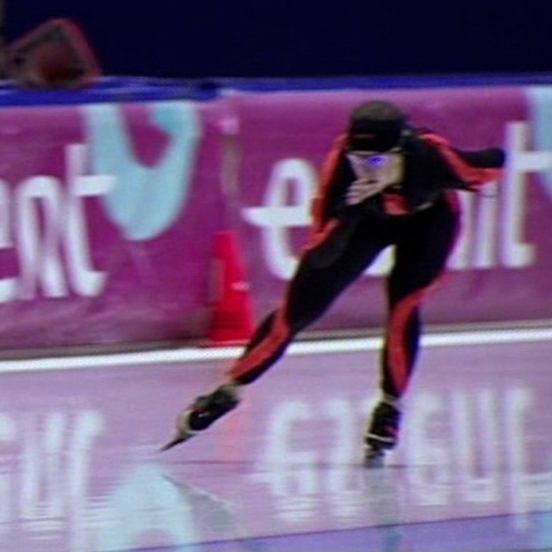
\includegraphics[width = 0.3\columnwidth]{figure6_4a}
	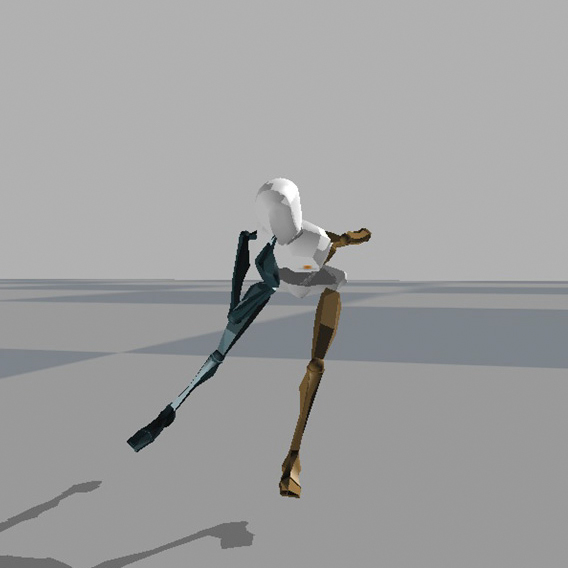
\includegraphics[width = 0.3\columnwidth]{figure6_4b}
	\label{fig:kappa-intro-applications-wust} 
  \caption{Left: Olympic and world champion speed skating Ireen W\"ust wearing sensors on her body. Right: graphical representation of the estimated orientation and position of her body segments.}
  \label{fig:appl-wust}
\end{figure}

In~\cite{kokHS:2014}, we present an algorithm for inertial motion capture which solves a smoothing optimization problem similar to~\eqref{eq:oriEst-posSmoothing}. A significant part of the model used in the algorithm in~\cite{kokHS:2014} is the state space model for pose estimation presented in~\eqref{eq:models-ssPose} and used in \Sectionref{sec:oriEst-poseEstimation}. This model is used for every sensor that is placed on the human body. The following adaptations are made to the model: 
\begin{description}[style=unboxed]
\item[Placement of the sensors on the body segments.]
The position and orientation of each sensor can be expressed in terms of its position and orientation on the corresponding body segment. Ideally, the sensor would be rigidly attached to the segment. However, it is physically impossible to place the sensor directly on the bone. Since it needs to be placed on the soft tissue instead, the sensor will inevitably move slightly with respect to the bone. We therefore model the position and orientation of each sensor on its corresponding body segment as 
approximately constant.
\item[Joints between the body segments.] A number of equality constraints enforce the body segments to be connected at the joint locations at all times. Note that equality constraints can straightforwardly be included in optimization problems \citep{boydV:2004,nocedalW:2006}.
\item[Exclusion of magnetometer measurements.] The magnetic field in indoor environments is not constant, see \eg \cite{ligorioS:2016}. This is specifically of concern in motion capture applications, since the magnetic field measured at the different sensor locations is typically different~\citep{luingeVB:2007,cooper:2009,favreJAA:2008,seelRS:2014}. Because of this, we do not include magnetometer measurements in the model. The inclusion of the equality constraints enforcing the body segments to be connected allows us to do so, since incorporating these constraints, the sensor's \textit{relative} position and orientation become observable as long as the subject is not standing completely still~\citep{hol:2011}.
\end{description}
As before, we denote the time-varying states by $x_t$ and the constant parameters by $\theta$. However, to highlight the different parts of the model, we split the states $x_t$ in states $x^{\text{S}_i}_t$ pertaining to the sensor $\text{S}_i$ and states $x^{\text{B}_i}_t$ pertaining to the body segment $\text{B}_i$, for $i = 1, \hdots , N_S$. Here, $N_S$ is the number of sensors attached to the body and it is assumed to be equal to the number of body segments that are modeled. Using this notation, the optimization problem that is solved in~\cite{kokHS:2014} can be summarized as
\begin{align}\label{eq:appl-optProblem-motionCapture}
\min_{x_{1:N},\theta} & \quad 
\underbrace{- \sum_{t = 2}^{N_T} \sum_{i = 1}^{N_S} \log p(x^{\text{S}_i}_t \mid x^{\text{S}_i}_{t-1})}_{\text{Dynamics of the state }x^{\text{S}_i}_t}
\underbrace{- \sum_{t = 1}^{N_T} \sum_{i = 1}^{N_S} \log p(x^{\text{B}_i}_t \mid x^{\text{S}_i}_{t})}_{\begin{subarray}{c}\text{Placement of sensor $\text{S}_i$}\\
    \text{on body segment $\text{B}_i$}\end{subarray}}
     \nonumber \\
& \hspace{20mm}\underbrace{- \sum_{i = 1}^{N_S} \log p(x^{\text{S}_i}_1) - \sum_{i = 1}^{N_S}\log p(\theta^{\text{S}_i})}_{\text{Prior}}
\nonumber \\
\st& \quad c(x_{1:N}) = 0,
\end{align}
where the number of time steps is denoted $N_T$ and $c(x_{1:N})$ denote the equality constraints from assuming that the body segments are connected at the joints. Note the similarities and differences between the structure of~\eqref{eq:appl-optProblem-motionCapture} as compared to~\eqref{eq:models-smoothingProbs} or~\eqref{eq:oriEst-posSmoothing}. The problem~\eqref{eq:appl-optProblem-motionCapture} is formulated as a smoothing algorithm. In \cite{miezalTB:2016}, a similar method is presented in which a sliding window approach is used to allow for online estimation. In \gls{ekf} formulations it is not straightforward to include equality constraints. However, as discussed in \cite{miezalTB:2016}, it is possible to include the equality constraints as a measurement update in the \gls{ekf} instead. 

Optionally, additional knowledge about the human body can be included in~\eqref{eq:appl-optProblem-motionCapture}. For instance, in \cite{kokHS:2014}, we include the knowledge that for some joints, it is known that their rotation is (mainly) limited to one or two axes. An example of this is the knee which is a hinge joint, although it can in practice flex a little around the other axes too. The optimization problem for that case would include a term that minimizes the rotation around certain axes. In \cite{taetzBM:2016}, a solution to the inertial motion capture problem is presented that includes additional biomechanical information. For instance, the shape of the body segments is approximated by a capsule and the sensors are assumed to be placed on the surface of the capsule. In~\cite{marcardRBP:2017}, the focus is instead on estimation of human motion using a much smaller amount of sensors. Because of the smaller number of sensors, the information about the human body and its motions is more crucial in their problem formulation. 

\section{Beyond pose estimation: activity recognition}
\label{sec:appl-actRecogn}
In this tutorial we have focused on position and orientation estimation using inertial sensors. A separate but related field of research is that of activity recognition using inertial sensors, where the aim is to determine the type of motion that is performed by a person wearing or carrying a device containing inertial sensors, see \cite{bullingBS:2014,avciBMMH:2010} for an overview. Since these sensors have become smaller, cheaper and more publicly available over the years, the amount of data that can be used for activity recognition has increased dramatically. For instance, inertial measurements collected from a smartphone can be used to classify daily activities. It is also possible to classify these activities using measurements from fitness and activity trackers, see \eg \cite{fitbit:2017,garmin:2017,polar:2017}. Standard activities which can be classified are for instance walking, running and sleeping, but there is a large number of other activities that one can think of as well. 

A simple example of activity recognition that is relevant for the motion capture application discussed in \Sectionref{sec:appl-motionCapture}, is footstep detection. As mentioned in \Sectionref{sec:appl-motionCapture}, the \emph{relative} position and orientation of the body can be determined using inertial sensors and a biomechanical model about the body segments being connected. However, the \emph{absolute} position can not be determined from this information. Because of that, it is not possible to determine if the subject is standing on the floor or floating in the air by only using the model~\eqref{eq:appl-optProblem-motionCapture}. Including the knowledge that during standing, walking and running, the feet are stationary on the floor during certain periods of time solves this problem \cite{foxlin:2005,colomarNH:2012}. It is possible to detect these stationary periods for example by identifying when both the angular velocity and the sensor's acceleration are approximately zero, see \cite{skogHNR:2010} for a comparison between different detection methods. The knowledge that the sensor is stationary can subsequently be included in~\eqref{eq:appl-optProblem-motionCapture} by adding a term to the cost function modeling the velocity of the sensor as being almost zero during these time periods. These are so-called zero velocity updates (ZUPTs)~\cite{foxlin:2005,colomarNH:2012}. 

Footstep detection is a very simple example where pose estimation can benefit from activity recognition. Another example is presented in~\cite{grzonkaDKB:2010} where maps of indoor environments are build using inertial measurements from sensors placed on the human body, very similar to the approach presented in \Sectionref{sec:appl-motionCapture}. In addition to the model presented in \Sectionref{sec:appl-motionCapture} and footstep detection, motions are detected of the subject opening and closing doors. Combining this information opens up for possibilities of performing \gls{slam}. In conclusion, activity recognition can serve as a source of additional information that can be included in our models for pose estimation. Conversely, in~\cite{hardeggerRCT:2016,reissHBS:2010} it is argued that activity recognition can also benefit from combination with pose estimation. 